


\begin{figure}[bt]
\centerline{
\includegraphics[width=8cm]{edge-samples-contrast}
}
\caption[The appearance of edges]{
%
The empirical appearance of edges.  Each $4\times 4$ grid represents
the possible appearance of an edge, quantized to just two luminance
levels.  The dark line centered in the grid is the average orientation
that patch was observed to have in the training data.
The upper set of patches are the most frequent ones that occur in
training data consisting of about 500 object segmentations.
The lower set of patches are a selection of patterns chosen to
illustrated the diversity of possible patterns that can occur.
The oriented features represented
include edges, thin lines, thick lines, zig-zags, corners
etc.  It is difficult to imagine a set of conventional
filters that could respond correctly to the full range of 
features seen here~-- all of which appeared multiple
times in object boundaries in real images.
%
}
\label{fig:seen-selected}
%%\label{fig:seen-selected-more}
\end{figure}


\ifnote
\begin{figure}[bt]
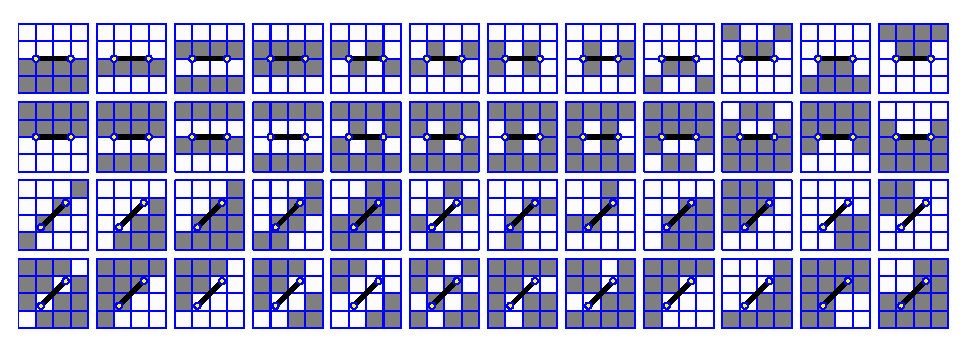
\includegraphics[width=\columnwidth]{seen-selected}
\caption
{
%
Edges have diverse appearances.  This figure shows 
the orientations assigned to a test suite
prepared by hand.  Each $4\times 4$ grid is a single test
edge patch, and the dark line centered in the grid is the orientation
that patch was observed to have in the training data.
The oriented features represented
include edges, thin lines, thick lines, zig-zags, corners
etc.  It is difficult to imagine a set of conventional
filters that could respond correctly to the full range of 
features seen here~-- all of which appeared multiple
times in object boundaries in real images.
%
}
\label{fig:seen-selected}
\end{figure}
\fi

\section{Building on segmentation}


As a specific example of development, the segmented views provided by
poking of objects and actors by poking can be collected and clustered
as shown in Figure~\ref{fig:clean-vision}.  Such views are precisely
what is needed to train up an object detection and recognition system,
and follow those objects and actors into other, non-poking contexts.

\begin{figure}[tb]
  \centerline{\includegraphics[width=10cm]{fig-poking-discovery}}
%%  \centerline{\includegraphics[width=\columnwidth]{fig-clean-vision}}
  \caption[How poking gets used]{
\label{fig:clean-vision}
%
The top row shows sample views of a toy car that the robot sees during
poking.  Many such views are collected and segmented as described
in~\protect\cite[]{fitzpatrick03first}.  The views are aligned to give an
average prototype for the car (and the robot arm and human hand that
acts upon it).  To give a sense of the quality of the data, the bottom
row shows the segmented views that are the best match with these
prototypes.  The car, the robot arm, and the hand belong to
fundamentally different categories.  The arm and hand cause movement
(are actors), the car suffers movement (is an object), and the arm
is under the robot's control (is part of the self).
%
}
\end{figure}

As well as giving information about the appearance of objects, the
segmented views of objects can be pooled to train up detectors for
more basic visual features~-- for example, edge orientation.  Once an
object boundary is known, the appearance of the edge between the
object and the background can be sampled along it, and labelled with
the orientation of the boundary in their neighborhood.
Figure~\ref{fig:seen-selected} shows an orientation filter trained up
from such data that can work at much finer scales than normally
possible when the filter is derived from an ideal edge model such as
that of \cite[]{chen00orientation}.  The ``catalog'' of edge appearances
found shows that the most frequent edge appearances is an ``ideal''
straight, noise-free edge, as might be expected (top of
Figure~\ref{fig:seen-selected})~-- but a remarkable diversity of other
forms also occur which are far less obvious (bottom of
Figure~\ref{fig:seen-selected}).

Can build on segmentation to learn about cool and useful stuff.

\subsection*{Learning about orientation}

A low-level example.

\subsection*{Learning to recognize objects}

A higher-level example.



\section{Learning about orientation}

Orientation is an important visual cue for many purposes, such as
object segmentation, recognition, and tracking.  It is associated with
neighborhoods rather than individual points in an image, and so is
inherently scale dependent.  At very fine scales, relatively few
pixels are available from which to judge orientation.
Lines and edges at such scales are extremely pixelated and
rough.
%
Orientation filters derived from analytic considerations, with
parameters chosen assuming smooth, ideal straight lines or edges (for
example, \cite{chen00orientation}) are more suited to larger
neighborhoods with more redundant information.
For fine scales, an empirical approach seems more promising, particularly
given that when the number of pixels involved is low, it is practical
to sample the space of all possible appearances of these pixels 
quite densely.

The data collected during segmentation allows us to explore how edges truly
look in ``natural'' images, by simply building up a catalog of edge
fragments seen around the boundaries of objects.  Of course, such a
catalog is only practical at small scales.  We worked with $4\times 4$
pixel windows, a size is chosen to be large enough to be interesting,
but small enough for the complete range of possible appearances to be
easily visualized.  Even at this scale, manual data collection and
labelling would be extremely tedious, so it is definitely advantageous
to have a robotic system to automatically compile and label a database
of the appearance of oriented features.
%
%, as shown in Figure~\ref{fig:separate-simple}.  
%Details of this procedure are given in
%Section~\ref{sect:experiment}.
These features were extracted by sampling image patches
along object boundaries, which were in turn determined 
using active segmentation.
The resulting catalog of edge appearances proved remarkably
diverse, although the most frequent appearances were indeed
the ``ideal'' straight, noise-free edge.

%Figures~\ref{fig:lines-all} and ~\ref{fig:seen-selected}.
%Figure~\ref{fig:seen-selected}.

\ifnote
\begin{figure}[tb]
\begin{center}
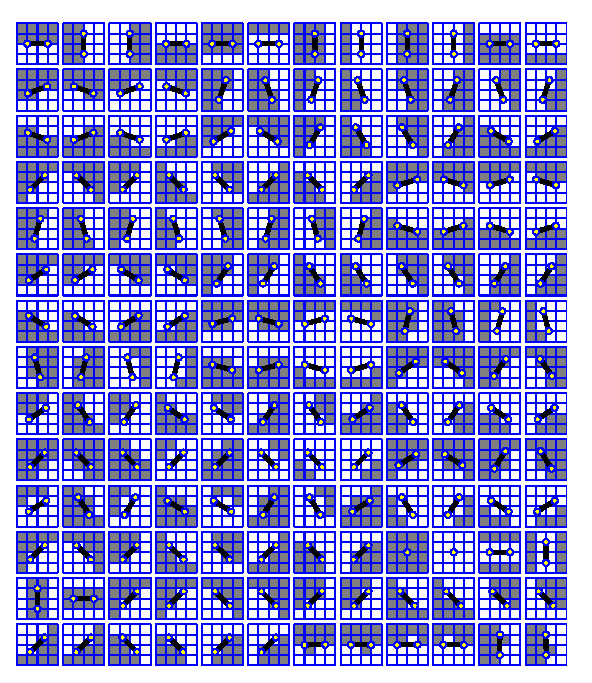
\includegraphics[width=\columnwidth]{seen-all}
\caption{
\label{fig:lines-all}
%
The most frequently observed edge appearances.  All patches
observed are replicated for all $90^{\circ}$ rotations, mirror flips,
and inversion of foreground/background.
%
The most frequent (top) are simple straight edges.
%
The line in the center of
each patch shows the orientation associated with that patch.  
%
After the straight edges, the completely empty patch
is common (produced in saturated regions), 
followed by a tube-like feature (third-last row)
where the boundary is visually distinct to either side of
the edge.
This is followed corner-like features and
many thousands of variations on the themes already seen.  
%
}
\end{center}
\end{figure}
\fi
